\documentclass[12pt]{article}

%PACKAGES
\usepackage{fullpage}
\usepackage{setspace}
\setlength{\parindent}{0cm}
\usepackage{parskip}
\usepackage{amssymb, amsmath, amsthm, graphicx}
\usepackage{mathtools}
\usepackage{siunitx}
\usepackage{comment}
\usepackage{scrextend}
\usepackage{lipsum}
\usepackage{float}

\newcommand\tab[1][1cm]{\hspace*{#1}}

%FONTS
\usepackage{times}

%COMMANDS
\newcommand{\note}[1]{\textcolor{orange}{#1}}
\DeclarePairedDelimiter{\norm}{\|}{\|}

\begin{document}
\begin{Large}
Human Guided Machine Vision for Road Detection\\
Team AddNameHereWhenWeFinallyDecide\\
\end{Large}
Kelsey DiPietro, Richard Frnka, Brian Hunter, Shaked Koplewitz, Khanh Nguyen, Scott Spencer

\subsection*{Problem Statement}

Detection of roads from an aerial view is an important problem, yet one with an elusive general solution. Road detection is essential to developing and maintaining a database of roads, especially with the increased use of GPS devices. Humans are particularly good at picking out roads from an image, but can only do so at a limited speed. Computers operate at the other end of the spectrum, lacking in a general algorithm to detect roads, but able to do so quickly. To get the best of both worlds, it is useful to combine a computer program with human input to fill in where a computer missed a road. 

$\newline$
The task was to create a program which finds roads in an aerial image and contains a user interface for a human to highlight specific roads and identify any missed roads. All user interface was to be done in a graphical component which allows the user to easily click on the image and have the computer do the rest of filling in and highlighting.

\subsection*{Initial Setup}
The project was divided into three subprojects: A pre-processing part which involved initially segmenting the image into candidate road component and an object detection part which involved ranking the components for their likeliness to be a road and finding obstructions that blocked view of the road. After pre-processing was complete, there was a graphical user interface piece which would allow a human user to select and highlight roads and identify any roads missed by the pre-processing.

All programming was done using MATLAB which has built in libraries for image segmentation and graphical user interface. Only simple images consisting of a single road with no cars were considered initially, but as the segmentation methods were developed, more complicated road configurations were used. Since no single algorithm performed well on all roads, many were considered, each with a unique segmentation process.

\subsection*{Segmentation Methods}

Below is a list of the segmentation functions with pseudocode and a brief description:


\subsubsection*{basicSegmentation}
\begin{addmargin}[12em]{1em}
	J $\leftarrow$ grayscale image \\
	BW $\leftarrow$ edge(J,canny) \\
	se0 $\leftarrow$ structural horizontal line of length 3 \\
	se90 $\leftarrow$ structural vertical line of length 3 \\
	BW $\leftarrow$ dilate(BW,[se0,se90]) \\
	BW2 $\leftarrow$ $\sim$BW \\
	BW, BW2 $\leftarrow$ fillHoles(BW), fillHoles(BW2)\\
	BW, BW2 $\leftarrow$ BW, BW2 minus small pieces \\
	CC1 $\leftarrow$ components(BW) \\
	CC2 $\leftarrow$ components(BW2) \\
	return CC1 + CC2 \\	
\end{addmargin}
This method is a bareboned road finder. It finds the edges, thickens them, fills the holes, cleans up noise, and returns the components.

\subsubsection*{blurSegmentation}
\begin{addmargin}[12em]{1em}
	J $\leftarrow$ grayscale image \\
	se $\leftarrow$ structural square \\
	Io $\leftarrow$ erode(J,se) \\
	Io $\leftarrow$ dilate(J,se) \\
	Ie $\leftarrow$ erode(Io,se) \\
	Iobr $\leftarrow$ reconstruct(Ie,$\sim$J) \\
	Iobrd $\leftarrow$ dilate(Iobr, se) \\
	blur1 $\leftarrow$ reconstruct($\sim$Iobrd,$\sim$Iobr) \\
	blur2 = $\sim$blur1 \\
	fgm, fgm2 $\leftarrow$ localmax(blur1), localmax(blur2) \\
	fgm, fgm2 $\leftarrow$ fillHoles(fgm), fillHoles(fgm2) \\
	CC1, CC2 $\leftarrow$ components(fgm), components(fgm2) \\
	return CC1 + CC2 \\
\end{addmargin}
This method blurs the image a significant amount to create a more even color distribution then looks for local maximums. It fills in any holes that were not local maxima and returns the components of the corrected image.

\subsubsection*{colorBasedSeg}
\begin{addmargin}[12em]{1em}
	J $\leftarrow$ grayscale image \\
	x,y $\leftarrow$ dimensions(J) \\
	blank $\leftarrow$ zeroMatrix(x,y) \\
	se $\leftarrow$ structural square \\
	Io $\leftarrow$ erode(J,se) \\
	Io $\leftarrow$ dilate(J,se) \\
	Ie $\leftarrow$ erode(Io,se) \\
	Iobr $\leftarrow$ reconstruct(Ie,$\sim$J) \\
	Iobrd $\leftarrow$ dilate(Iobr, se) \\
	Iobrcbr $\leftarrow$ reconstruct($\sim$Iobrd,$\sim$Iobr) \\
	CC $\leftarrow$ components(null) \\
	for i in range 0 to 255: \\
	\tab C $\leftarrow$ Iobrcbr == i \\
	\tab C $\leftarrow$ fillHoles(C) \\
	\tab C $\leftarrow$ C minus small pieces \\
	\tab C $\leftarrow$ components(C) \\
	\tab for j in range 1 to length(C): \\
	\tab\tab CC += C \\
	\tab rof \\
	rof \\
	return CC \\	
\end{addmargin}
Similar to blurSegmentation, this method first blurs the image to get a more even color distribution. It then gets components by taking pixels of each color index, filling the holes, cleaning up noise, and merging them into one component list to return.

\subsubsection*{Connected\_Comp\_Edges}
\begin{addmargin}[12em]{1em}
	I $\leftarrow$ grayscale image \\
	hy $\leftarrow$ sobelFilter \\
	Iy $\leftarrow$ filter(I,hy) \\
	Ix $\leftarrow$ filter(I,hy') \\
	se $\leftarrow$ structural square \\
	Io $\leftarrow$ dilate(J,se) \\
	Io $\leftarrow$ erode(J,se) \\
	Ie $\leftarrow$ erode(Io,se) \\
	Iobr $\leftarrow$ reconstruct(Ie,$\sim$J) \\
	Iobrd $\leftarrow$ dilate(Iobr, se) \\
	Iobrcbr $\leftarrow$ reconstruct($\sim$Iobrd,$\sim$Iobr) \\
	fgm $\leftarrow$ localmax(Iobrcbr) \\
	fgm $\leftarrow$ edge(fgm,sobel) \\
	fgm $\leftarrow$ thicken(fgm) \\
	se $\leftarrow$ structural disk \\
	cfgm $\leftarrow$ erode(fgm,se) \\
	cfgm $\leftarrow$ dilate(cfgm,se) \\
	inv $\leftarrow$ $\sim$cfgm \\
	CC $\leftarrow$ components(inv) \\
	return CC \\		
\end{addmargin}
A method that uses a Sobel filter and multiple dilations an erosions to smooth an image. It finds the edges using the Canny method and thickens them before finding the components.

\subsubsection*{majorSegmentation/ImageSegmentation}
\begin{addmargin}[12em]{1em}
	rgb $\leftarrow$ color image \\
	rgbblur $\leftarrow$ gaussFilter(rgb) \\
	gray $\leftarrow$ grayscale(rgbblur) \\
	edges $\leftarrow$ edge(gray, Canny)\\
	edges $\leftarrow$ thicken(edges)\\
	structElem $\leftarrow$ structural square\\
	edges $\leftarrow$ dilation(edges, structElem)\\
	edges $\leftarrow$ erosion(edges, structElem)
	edges $\leftarrow$ shrink(edges)\\
	edges $\leftarrow$ \~edges\\
	bw $\leftarrow$ BW image with non-roads blacked out\\
	bwEdged $\leftarrow$ edges .* bw\\
	filt $\leftarrow$ bwEdged minus small pieces\\
	filt $\leftarrow$ thicken(filt)\\
	filt $\leftarrow$ fillHoles(filt)\\
	
	return components(filt)\\
\end{addmargin}
This method enhances external boundaries, darkens internal boundaries, and uses Canny edge detection to split the image up into components. This algorithm is used in the GUI as this tended to be the most robust segmentation algorithm. The GUI also uses two other algorithms which are modifications of this one, and in the performance table below, this general algorithm is simply referred to as ImageSegmentation.

\subsubsection*{ext\_grad\_seg}
\begin{addmargin}[12em]{1em}
	ibw $\leftarrow$ grayscale image \\
	se $\leftarrow$ structural square \\
	eg $\leftarrow$ dilate(ibw,se) - ibw \\
	rec $\leftarrow$ reconstruct(eg,ibw) \\
	f1 $\leftarrow$ edge(rec,canny) \\
	fgm $\leftarrow$ localmax(rec) \\
	fgm $\leftarrow$ fgm minus small pieces \\
	return components(fgm) \\
\end{addmargin}
This method enhances external boundaries, darkens internal boundaries, and uses Canny edge detection to split the image up into components.

\subsubsection*{rgbSeg}
\begin{addmargin}[12em]{1em}
	J $\leftarrow$ color image \\
	x,y $\leftarrow$ dimension(J) \\
	apform $\leftarrow$ L*a*b form of J \\
	apd $\leftarrow$ reshape apform to x*y by 2 \\
	cluster $\leftarrow$ kmeans(apd) with k = 5 \\
	pixels $\leftarrow$ reshape cluster to x by y \\
	CC $\leftarrow$ empty component list \\
	for i in range 1 to 5: \\
	\tab temp $\leftarrow$ x by y zero matrix \\
	\tab temp $\leftarrow$ fillHoles(temp) \\
	\tab temp $\leftarrow$ (pixels == i) minus small pieces \\
	\tab CC += components(temp) \\
	rof \\
	return CC \\
\end{addmargin}
This method takes an rgb image and segments it into 5 parts using k-means. It then finds components for each individual cluster and merges them together in a master list. 

\subsubsection*{thinRoad}
\begin{addmargin}[12em]{1em}
	I $\leftarrow$ grayscale image \\
	I2 $\leftarrow$ $\sim$I \\
	x,y $\leftarrow$ dimensions of I \\
	BW1, BW2 $\leftarrow$ I $>$ 150, I2 $>$ 150 \\
	BW1, BW2 $\leftarrow$ fillHoles(BW1), fillHoles(BW2) \\
	BW1, BW2 $\leftarrow$ BW1, BW2 minus very small pieces \\
	CC1, CC2 $\leftarrow$ components(BW1), components(BW2) \\
	return CC1 + CC2 \\
\end{addmargin}
This method segments a grayscale image and it's complement by separating by intensity and filling holes. It removes only very small components to accommodate for the small area of thin roads.

\subsection*{Computational Efficiency Comparison}

All the above segmentation methods produce different connected component matrices, to varying levels of accuracy. We ran each algorithm separately and took note of the computational time required for each method, the number of connected components, and, using a very rough visual test, we measured the overall ability of each algorithm to detect the roads in an efficient manner. 

All tests were ran using MATLAB2014b, on a standard laptop. It should be noted though that these times only reflect the computational time required for preprocessing. If an image is segmented properly, than the GUI runs very close to real time with little processing time. Therefore, we will take identifying all the roads properly for longer computational time over poor road identification and shorter preprocessing time. 


We use the following two test images: 
\begin{figure}[h!]
  \centering
  \begin{minipage}[b]{0.4\textwidth}
    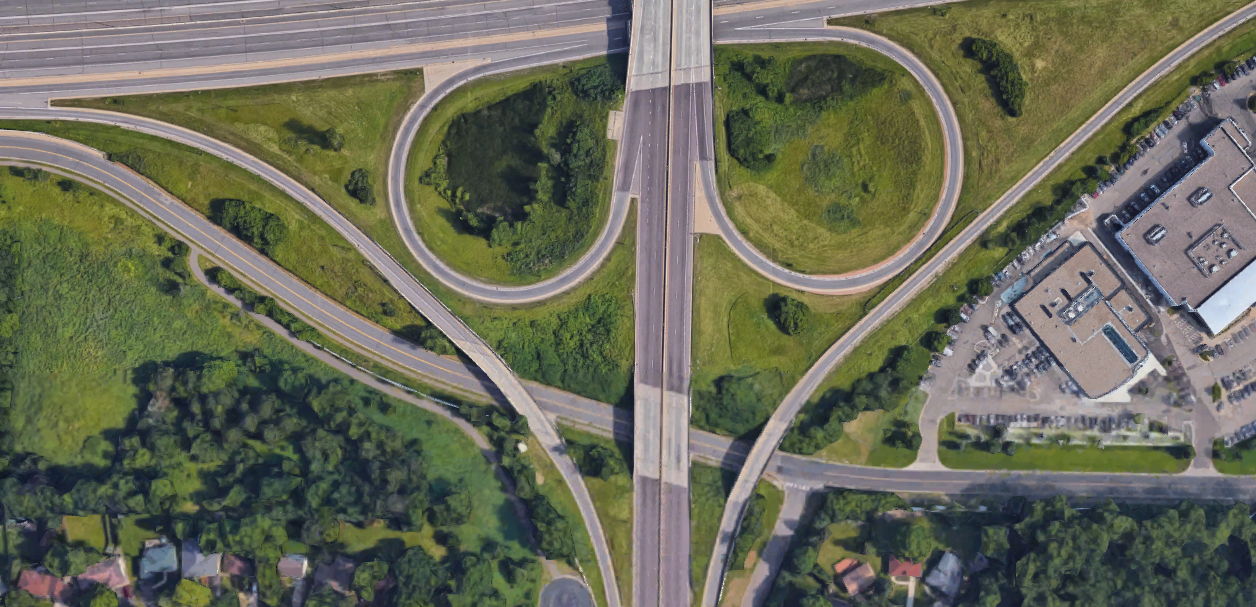
\includegraphics[width=\textwidth]{1004.png}
    \caption{Highway Image}
  \end{minipage}
  \hfill
  \begin{minipage}[b]{0.4\textwidth}
    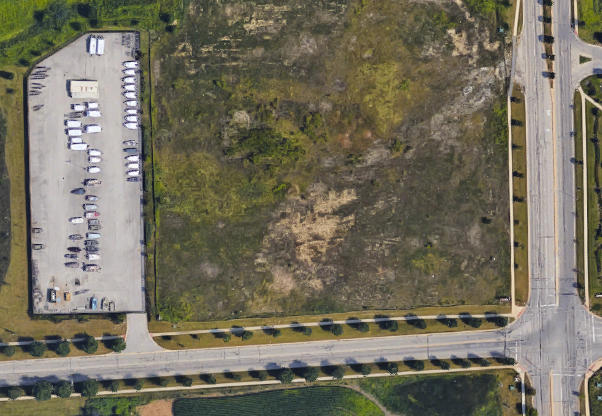
\includegraphics[width=\textwidth]{roadnearlot.png}
    \caption{Residential Image}
  \end{minipage}
\end{figure}

The following two tables generalize our results. While the ImageSegmentation filter takes the longest, it correctly identifies all the roads for both images based on a crude visual analysis. While the other algorithms have a shorter computational time, they either miss key road segments or add a lot of additional noise to the connected road components, which would increase the processing time for GUI component of the project. Therefore we strictly use the ImageSegmentation filter for all of our test cases. 

\begin{figure}[h!]
\centering
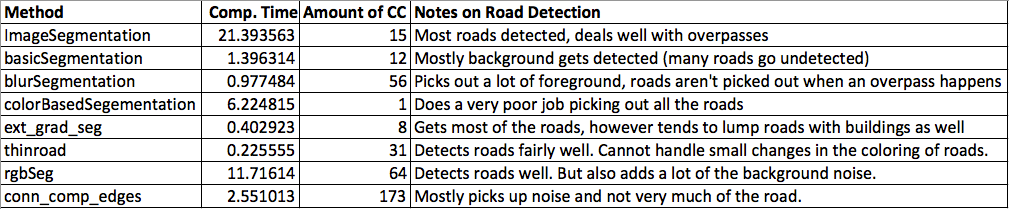
\includegraphics[scale = 0.4]{image1table.png}
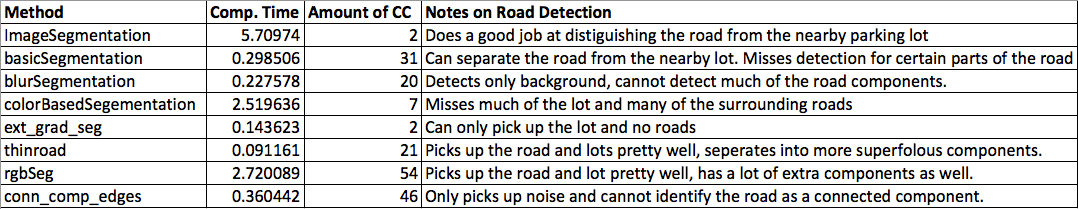
\includegraphics[scale = 0.4]{image2table.png}
\end{figure}

Future work would entail doing some kind of weighted average using the best algorithms and implementing them for our test images. Also, as the charts show, some segmentation strategies work better for highway systems than they do for more residential areas, which is why we used the ImageSegmentation for our examples, as it performs robustly on both within the preprocessing step. 

\subsection*{Canny Edge Detection and K-Means}
Canny edge detection comes up frequently in the segmentation methods above. This edge detection algorithm has six steps, which are outlined here: Apply a Gaussian filter to reduce unwanted noise, compute the gradient of the image, finding an optimal cutoff threshold and apply it to the image, suppress non-maxima pixels, threshold the image twice more with a low and high threshold, and merge segments in the noisier image using the low noise image as a guide. MATLAB does feature many other edge detection algorithms, but Canny was found to be a strong candidate for road detection due to it's ability to suppress unwanted noise and find the true edge of the road. 

$\newline$
The rgbSeg method used the k-means algorithm from machine learning as a way to divide an image by it's color value. K-means works by first assigning k random centroids among the set of data points, in this case pixels. Then at each step, every point is assigned to the group which has the closest centroid and after all points are grouped, new centroids are calculated. New group assignments and centroids are found until the groups stop changing, at which point the algorithm has converged to a local minimum. It is important to note that k-means will converge to a local minimum, but it is not guaranteed to be a global minimum. Depending on the amount of pre-processing time allowed, it may be beneficial in the rgbSeg method to repeat the k-means method multiple times and take the best solution, as this could help to ensure that the image is not segmented into an undesirable local minimum. However, in practice, a non-optimal clustering on the image did not hinder road detection to a significant extent in that if any additional pieces were grouped in the same cluster as the road, they were separated when splitting up the image into components.



\subsection*{User Interface}
\indent The Graphical User Interface (GUI) provides a way to interact with the project without having to sort through the code or do any kind of programming. Ideally, this would be presented to a client so they can point and click without worrying about any of the background processing. 
\\
\indent Initially, the user loads whatever image they would like to analyze. Any new image that is loaded should clear the current process and refresh the interface. Once an image is loaded, pre-processing is done in the background. This runs the default segmentation (Major Segmentation) behind the scenes, and produces the components that are used throughout the rest of the program. The user sees a message box implying patience that vanishes once initialization is complete.
\\
\indent After pre-processing, the user can begin to interact with the rest of the GUI. One of the more helpful features is the Show All Roads button. This shows the results of the image segmentation method that is being used and gives a visual clue as to what can be considered a road. The user can check the Select Roads box to begin drawing their path. The GUI keeps track of what roads have been selected with a binary vector $X$, which is the size of the number of components. $X$ is updated as users click on the components they want, and it is one of the major global paremeters that is passed through the GUI. With X and the component cell CC, it is easy to highlight the selected roads in the image by turning all of the pixels corresponding to selected components blue (0000FF).
\\
\indent The GUI has options to clear the current image and its parameters, save the file by exporting the current image to a new PNG, change the segmentation method to the options indicated above, and turn on shadow detection. The current shadow detection has thresholds adjusted to fit certain images, but ideally, the user could adjust these parameters in the future. \\
Included below are two pictures of the GUI in action. It loads the image and runs the pre-processing image segmentation to get the road components. As shown in the second image, it allows the user to select which roads to highlight. In the example, the user has selected the left and right roads, but has left the center road unselected. 

\begin{figure}[H]
	\centering
	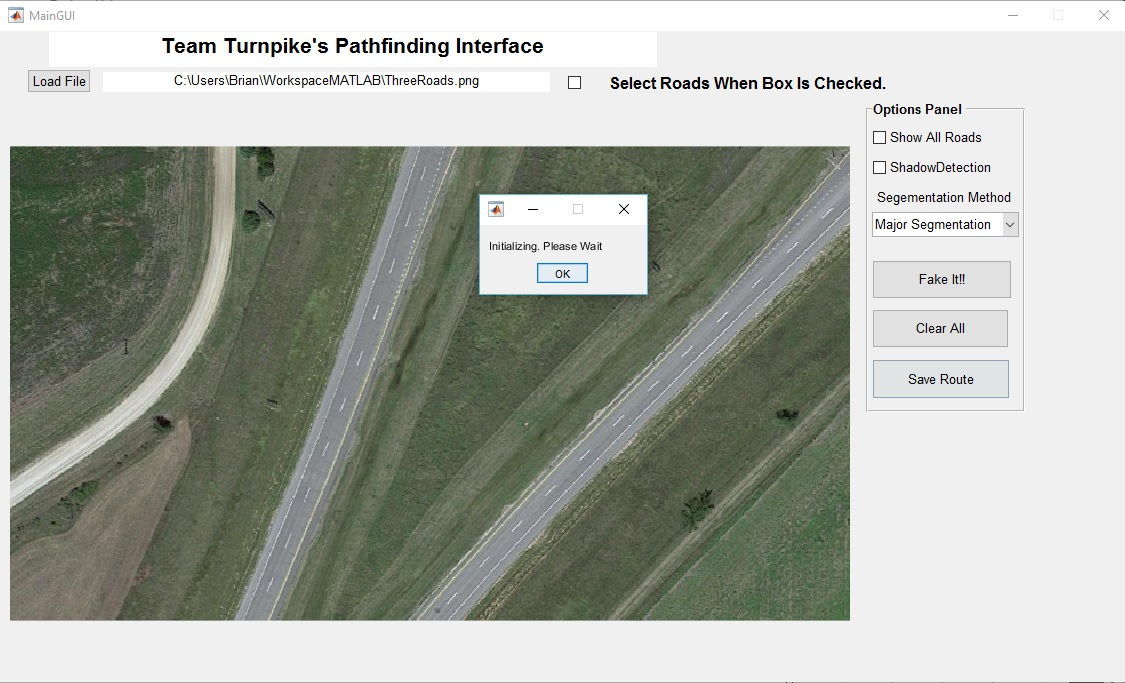
\includegraphics[scale = 0.5]{GUI1.jpg} \\
	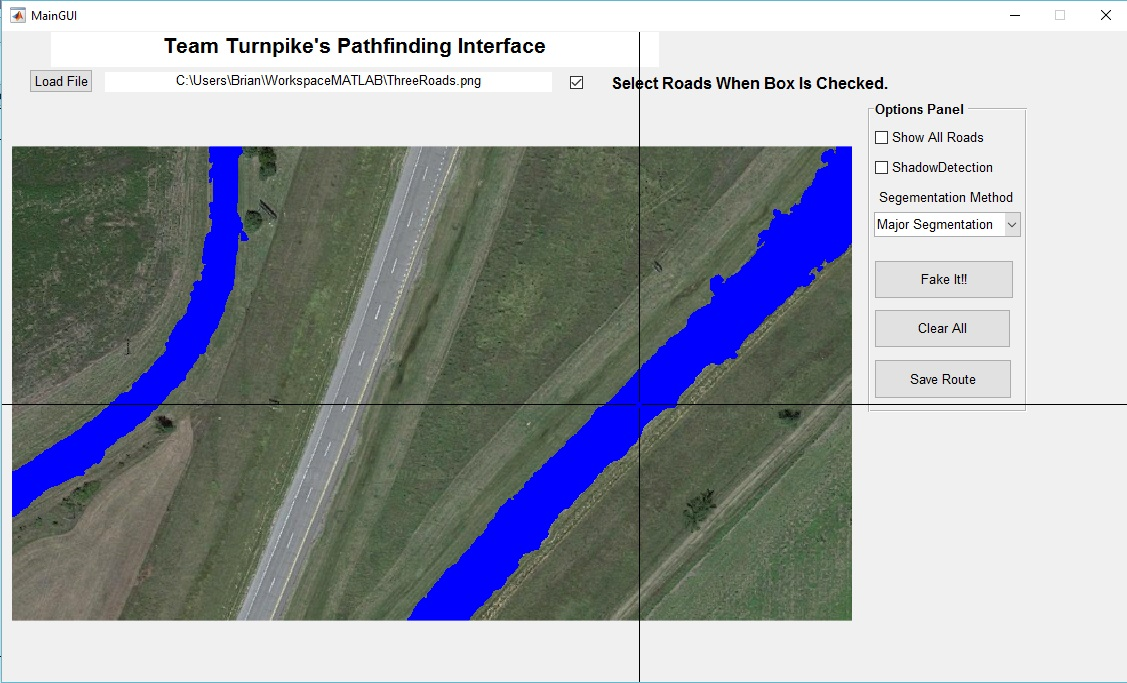
\includegraphics[scale = 0.5]{GUI2.jpg}
\end{figure}

\subsection*{Object and Road Detection}
%TODO: (Shaked)

\subsubsection*{car\_detection}
\begin{addmargin}[12em]{1em}
	M1\_B $\leftarrow$ grayscale image \\
	M2\_B $\leftarrow$ maximum intensity of each row of M1\_B \\
	T1\_B $\leftarrow$ mean(M2\_B) \\
	T2\_B $\leftarrow$ min(M2\_B) \\
	T3\_B $\leftarrow$ mean(T1\_B,T2\_B) \\
	Image1\_B $\leftarrow$ 0 if M1\_B(i,j) \textless T1\_B; 1 if M1\_B(i,j) \textgreater T1\_B \\
	Image2\_B $\leftarrow$ 0 if M1\_B(i,j) \textless T2\_B; 1 if M1\_B(i,j) \textgreater T2\_B \\
	Image3\_B $\leftarrow$ 0 if M1\_B(i,j) \textless T3\_B; 1 if M1\_B(i,j) \textgreater T3\_B \\
	New\_Image1\_B $\leftarrow$ bitand(Image1\_B, Image2\_B) \\
	New\_Image2\_B $\leftarrow$ bitand(New\_Image1\_B, Image3\_B) \\
	Bright\_cars $\leftarrow$ bitor(New\_Image1\_B, New\_Image1\_B) \\
	M1\_D $\leftarrow$ grayscale image \\
	M2\_D $\leftarrow$ minimum intensity of each row of M1\_D \\
	T1\_D $\leftarrow$ mean(M2\_D) \\
	T2\_D $\leftarrow$ min(M2\_D) \\
	T3\_D $\leftarrow$ mean(T1\_D,T2\_D) \\
	Image1\_D $\leftarrow$ 1 if M1\_D(i,j) \textless T1\_D; 0 if M1\_D(i,j) \textgreater T1\_D \\
	Image2\_D $\leftarrow$ 1 if M1\_D(i,j) \textless T2\_D; 0 if M1\_D(i,j) \textgreater T2\_D \\
	Image3\_D $\leftarrow$ 1 if M1\_D(i,j) \textless T3\_D; 0 if M1\_D(i,j) \textgreater T3\_D \\
	New\_Image1\_D $\leftarrow$ bitand(Image1\_D, Image2\_D) \\
	New\_Image2\_D $\leftarrow$ bitand(New\_Image1\_D, Image3\_D) \\
	Dark\_cars $\leftarrow$ bitor(New\_Image1\_D, New\_Image1\_D) \\
	cars $\leftarrow$  bitor(Dark\_cars,Bright\_cars) \\
	CC $\leftarrow$ bwconncomp(cars) \\
	car\_labels $\leftarrow$ labelmatrix(CC) \\
	return car\_labels \\
\end{addmargin}
Inspired by the idea of Sumalatha Kuthadi's master's thesis, this method finds bright colored cars and black colored cars using multiple thresholds. Bright colored cars' intensities are higher comparing to roads' intensity, and dark colored cars' intensities are lower comparing to roads' intensity. Both types of cars are combined to define all cars on the road. This method successfully determines all cars in a parking lot. Unfortunately, it won't work in more complicated pictures because it will focus on any other objects with brighter colors or darker colors as cars. As a result, this is not used in the implementation of the main algorithm.

$\newline$
Shadow detection code was written by Beril Sirmacek, and is permitted to redistribute and use in source code. This code was used in the algorithm listed in future work to remove shadows from images.

\subsection*{Code Call Chart}
The GUI serves as the main function with which the user can interface. Since each segmentation function was made to run as it's own independent component, the GUI can make calls to any and all of these, and each function is self-contained. The GUI currently makes use of simpleSegmentation, majorSegmentation, and overpassSegmentation. The majorSegmentation algorithm is listed above and the other two methods are slight variations of it. Additionally, the GUI also calls shadows, showAllRoads, and selectedRoads to highlight various areas on the image. This yields a simple call chart displayed below. 
\begin{figure}[h!]
	\centering
	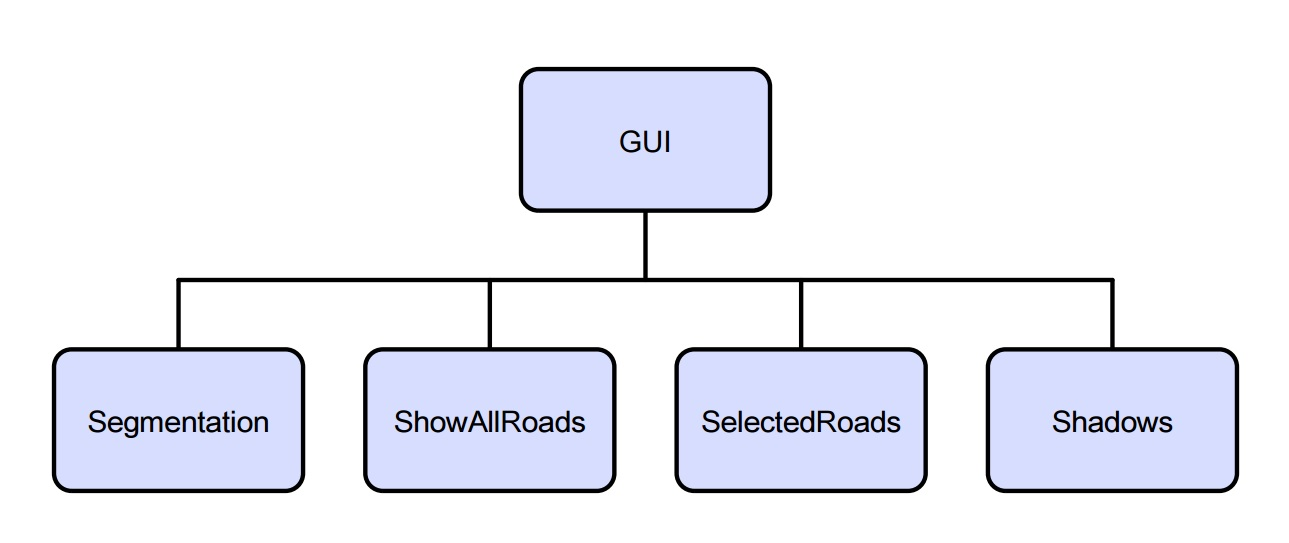
\includegraphics[scale = 0.5]{callChart.jpg}
\end{figure}

For the shadow removal, shadow\_detect served as the main method which called removeShadows to modify the image. Shadow detection is used in the GUI as the function shadows, mentioned above, but the removal function has not yet been included. Given the simplicity of a single main and function file, the call chart for these two is omitted.

\subsection*{Future Work}
Our methods were able to properly segment and detect road paths for a narrow sample of test images. This sample includes roads without shadows, highway systems with simple inter-passes, and intersections where there is a strong change in intensity between the intersecting roads. An example of the later category is an intersection where the main road has been recently repaved, thus darker, than its corresponding intersection road. In addition, we chose to sample images from the same satellite scaling (i.e. a scale of 100 ft from Google Earth aerial view). 

If given more time, we would like to extend our implementation to a wider host of sample problems. These future directions as well as possible strategies for tackling these more complications are given below. 

\begin{enumerate}
\item Car detection and removal: For our sample images, we considered roads that only had a few cars. Because the scale of the car was much smaller than the road, our algorithm was able to ignore the car and still return a connected component road. We would like to extend our algorithm to identifying roads that have more traffic on them, which would interfere with the connectivity of the segmentation. Ideally, we would be able to identify (using size training algorithms) all the cars in the image and either remove those cars or change them to the color of the road. This would allow for the segmentation algorithm to still see the road as a connected component to highlight, regardless of the traffic. 
\item Shadow detection and removal: Similar to cars with high traffic, shadows pose a huge obstruction to our algorithm's ability to perform. Often times shadows from trees and buildings end up breaking up the road in separate connected components. Similar to the car detection, ideally we would use filter that could identify all shadows on the roads and change those shadows to the same intensity of the road and then feed that image to the segmentation component of our preprocessing algorithm. We have been able to do this for small shadows that only obscure part of the road, but have not been able to remove larger shadows that segment much of the road. 

$\newline$
Below is pseudocode for the shadow removal algorithm. It works by going around the boundary of detected shadows and dilates over points within 2 units to the left, right, above, and below. After dilating the boundary points, it finds the boundary of the new, smaller shadow and continues this process until all points of the shadow have been covered.

\begin{addmargin}[12em]{1em}
	gr,gg,gb $\leftarrow$ r,g,b components of image \\
	gr,gg,gb $\leftarrow$ gr,gg,gb embedded in a larger matrix \\
	blank $\leftarrow$ bw matrix with only shadows \\
	x,y $\leftarrow$ x,y coordinates of boundary pixels of shadows \\
	while x,y not empty \\
	\tab for i in range of length of x \\
	\tab\tab dilate gr,gg,gb at point x[i],y[i] \\
	\tab rof \\
	\tab blank $\leftarrow$ blank minus boundary points \\
	\tab x,y $\leftarrow$ coordinates of boundary pixels in blank \\
	elihw
	nosh $\leftarrow$ inner matrices of gr,gg,gb combined\\
	return nosh
\end{addmargin}

Included as an example is an image in which a shadow partially obstructs the view of the road. Shadows identified by the shadow detection method are highlighted in blue, and below is the result after the above function is run.

\begin{figure}[H]
	\centering
	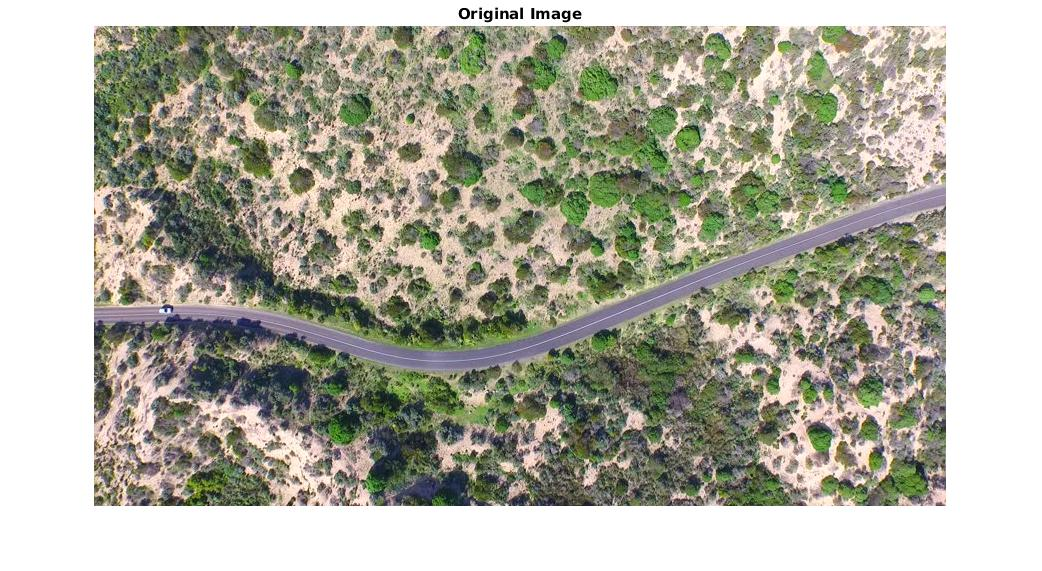
\includegraphics[scale = 0.3]{singleroad1.jpg}
	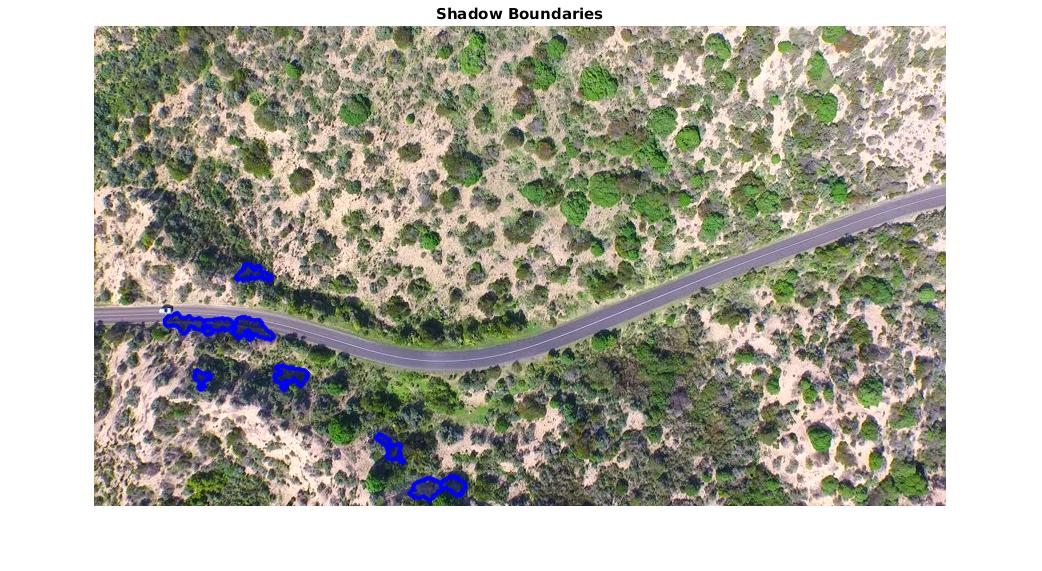
\includegraphics[scale = 0.3]{shadowBoundaries.jpg}
	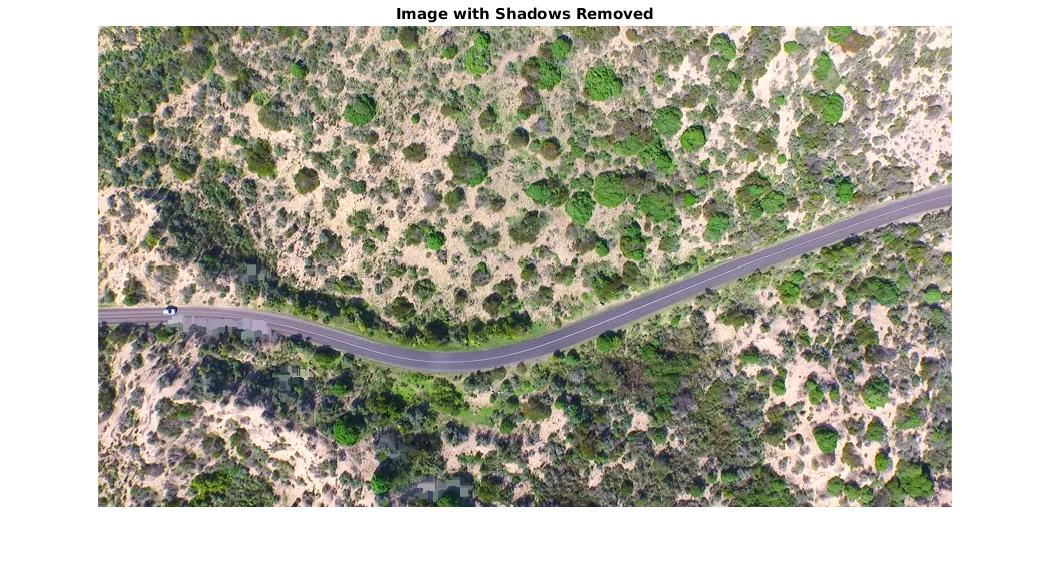
\includegraphics[scale = 0.3]{shadowFixed.jpg}
\end{figure}

\item Extending the road detection algorithm: Currently our road detection takes connected components from image segmentation and returns the probability that each component is a road. This allows for limited processing to be wasted in the GUI if the user clicks a large connected component such as a forest. It would be helpful to add an additional component to this algorithm that would work in conjunction with the GUI, so that if the user clicks within some region nearby the road, it will take them to the nearest road. 
\item Detecting intersections and choosing directions: Our algorithm can only handle intersections in which there is a change in the intensity between intersecting roads. Ideally, we would want to be able to handle any type of intersection. Finding and segmenting an intersection consists of two parts: identifying the fact that we are at an intersection and segmenting that intersection into its component parts. 
	\begin{enumerate}
	\item Identifying an intersection: Intersection identification could be done a local level for the given image. Given road segmentation, one could find an intersection by looking at the width of the road (which should stay constant). At an intersection, this constant width changes and the location of this change should be flagged as an intersection. 
	\item Breaking up the intersection: once a location is flagged as an intersection point, create lines in each direction of the intersection that cause an intensity change. This is equivalent to building a new edge, so that the algorithm detects the edge and breaks up the connected road component.  
	\end{enumerate} 
\end{enumerate}



\end{document}

